\chapter{Scaling behaviour of generalised SIAM: low energy effective theories}
\label{fullurg}

\section{RG equations}
The RG equations have already been derived, we repeat them here for convenience:
\begin{gather}
	\Delta U = 4V^2 n_j\left(\frac{1}{d_1} - \frac{1}{d_0}\right) - n_j\left(\frac{J^2}{d_2} - \frac{K^2}{d_3}\right),\\
	\Delta V = -\frac{3n_j V}{8}\left[J\left(\frac{1}{d_2} + \frac{1}{d_1}\right) + K \left(\frac{1}{d_3} + \frac{1}{d_0}\right)\right],\\
	\Delta J = -\frac{n_j J^2}{d_2}, \quad\quad\Delta K = -\frac{n_j K^2}{d_3}
\end{gather}
We have assumed the impurity levels are particle-hole symmetric (\(\epsilon_d = -\frac{U}{2}\)), and the denominators are given by
\begin{equation}\begin{aligned}
	d_0 = \omega - \frac{D}{2} - \frac{U}{2} + \frac{K}{4}, \quad d_1 = \omega - \frac{D}{2} + \frac{U}{2} + \frac{J}{4}, \quad d_2 = \omega - \frac{D}{2} + \frac{J}{4}, \quad d_3 = \omega - \frac{D}{2} + \frac{K}{4}
\end{aligned}\end{equation}

\section{Nature of RG flows: \(U>0\)}
For the Hamiltonians with positive on-site correlation, we will assume that the spin-exchange coupling is positive and charge isospin-exchange coupling is negative: \(J>0, K<0\). This choice is motivated by the signs of the corresponding terms when they are generated via a Schrieffer-Wolff transformation~\cite{schrieffer1966}. The impurity-bath hybridisation \(V\) is always positive.

We will in general assume that \(\omega < 0\). The strong-coupling regime is defined as the range of values of \(\omega\) where the hybridisation is relevant. This is ensured by the assumption \(d_1<0\). Note that since \(d_2 < d_1\) for \(U>0\), the assumption of \(d_1 < 0\) also ensures that \(d_2 < 0\). The assumptions of \(\omega < 0\) and \(K < 0\) also mean \(d_0 < 0, d_3 < 0\). In summary, all the denominators are negative: \(d_i = -|d_i|\). The simplest consequence of this is the RG flow of \(K\):
\begin{equation}\begin{aligned}
	\Delta K= -\frac{n_j K^2}{d_3} = \frac{n_j K^2}{|d_3|} > 0 \implies K_{j+1} > K_j \implies K_0 = -|K_0|, K^* \to 0
\end{aligned}\end{equation}
\(K_j\) is the value of \(K\) after the \(j^\text{th}\) RG step, \(K_0\) representing the bare value.
In other words, since \(d_3 < 0\), the RG equation for \(K\) provides an algebraic increment, and the negative \(K\) increases and flows towards zero. The \(*\) indicates a fixed point value. The isospin coupling is irrelevant in this regime, and we will ignore it.

The coupling \(J\), on the other hand, is relevant and flows from a small positive value towards a large value at strong-coupling.
\begin{equation}\begin{aligned}
	\Delta J= -\frac{n_j J^2}{d_2} = \frac{n_j J^2}{|d_2|} > 0 \implies J_{j+1} > J_j \implies J_0 \to \text{ large } J^* ~(\text{strong-coupling})
\end{aligned}\end{equation}
The value of \(J^*\) is obtained when the denominator \(d_2\) vanishes.

Because of the RG irrelevance of \(K\), we can simplify the RG equation for \(V\):
\begin{equation}\begin{aligned}
	\Delta V = -\frac{3n_j VJ}{8}\left(\frac{1}{d_2} + \frac{1}{d_1}\right) = \frac{3n_j VJ}{8}\left(\frac{1}{|d_2|} + \frac{1}{|d_1|}\right) > 0
\end{aligned}\end{equation}
Since both the denominators are positive, \(V\) is relevant. The fixed point value \(V^*\) is attained when the denominator \(d_1\) vanishes (\(d_1\) will vanish earlier than \(d_2\)).

We can compare the rate of flows of \(V\) and \(J\):
\begin{equation}\begin{aligned}
	\frac{\Delta V}{\Delta J} = \frac{3V}{8J}\left(1 + \frac{|d_2|}{|d_1|}\right) > \frac{3V}{4J}
\end{aligned}\end{equation}
There we used the fact that \(|d_2| > |d_1|\).

We finally come to the RG equation for \(U\):
\begin{equation}\begin{aligned}
	\Delta U = 4V^2 n_j\left(\frac{1}{d_1} - \frac{1}{d_0}\right) - n_j\frac{J^2}{d_2} = -4V^2\left(U + \frac{J}{4}\right)\frac{n_j}{d_0 d_1} - \frac{n_j J^2}{d_2}
\end{aligned}\end{equation}

For \(V>J\), we can expect \(U\) to be irrelevant. On the other hand, \(V<J\) will make \(U\) irrelevant.

\begin{figure}[htpb]
	\centering
	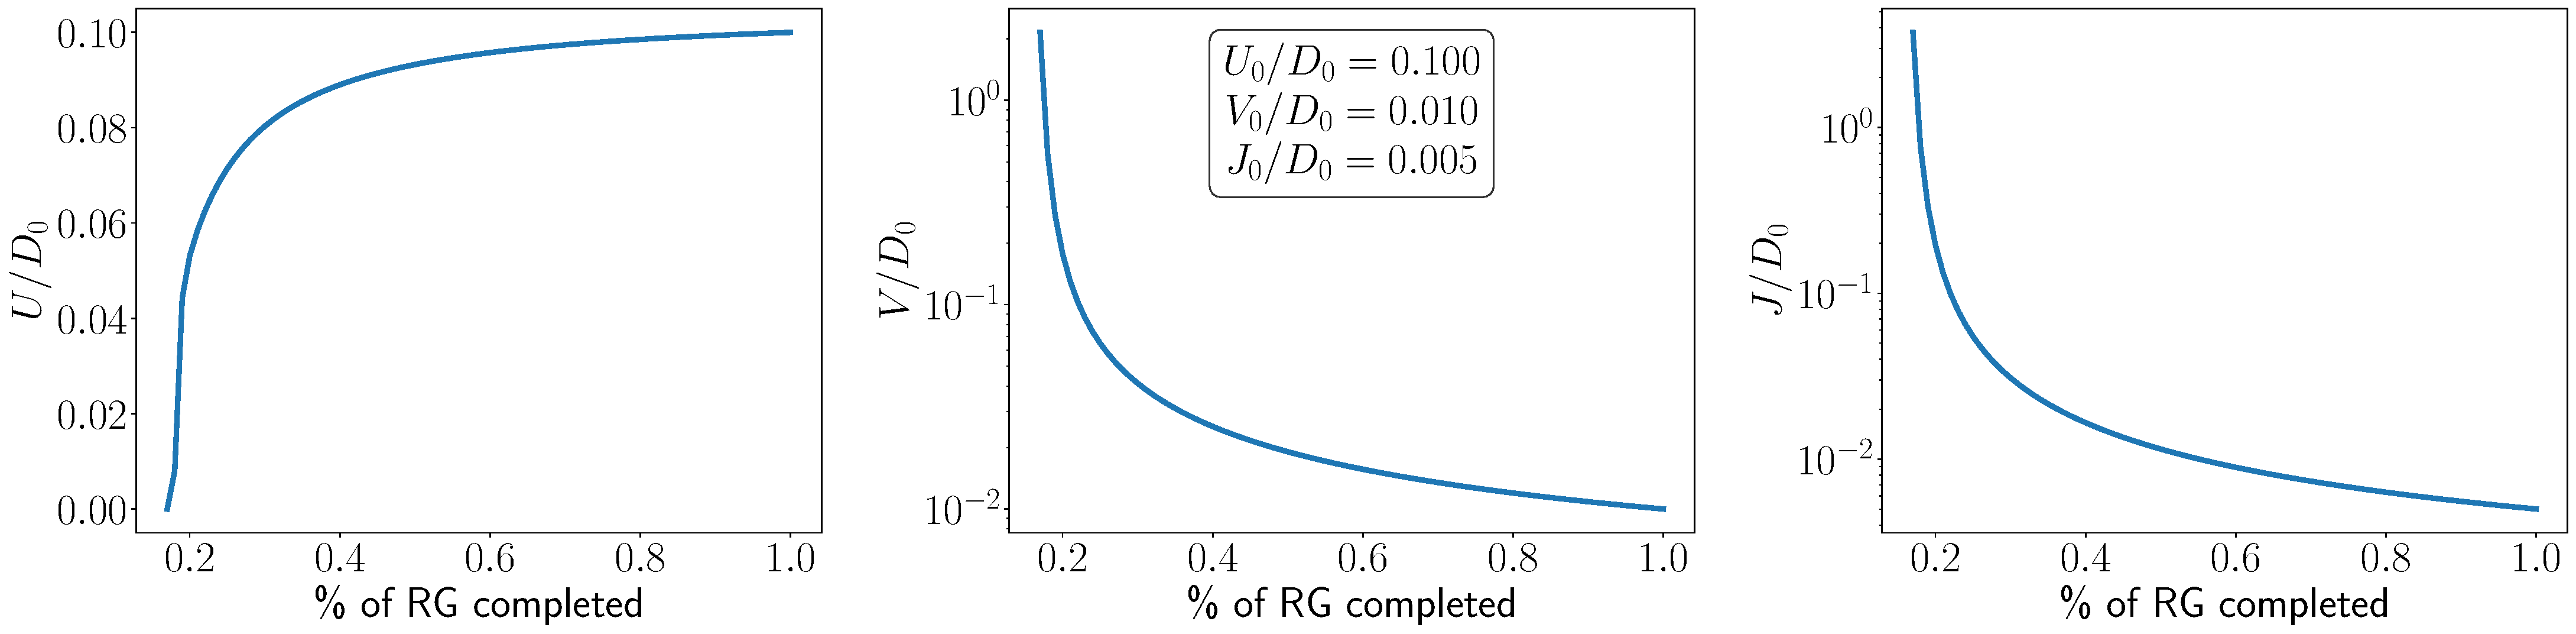
\includegraphics[width=0.99\textwidth]{../spin-charge-symmetrical/U_irr,U_gt_0.pdf}
	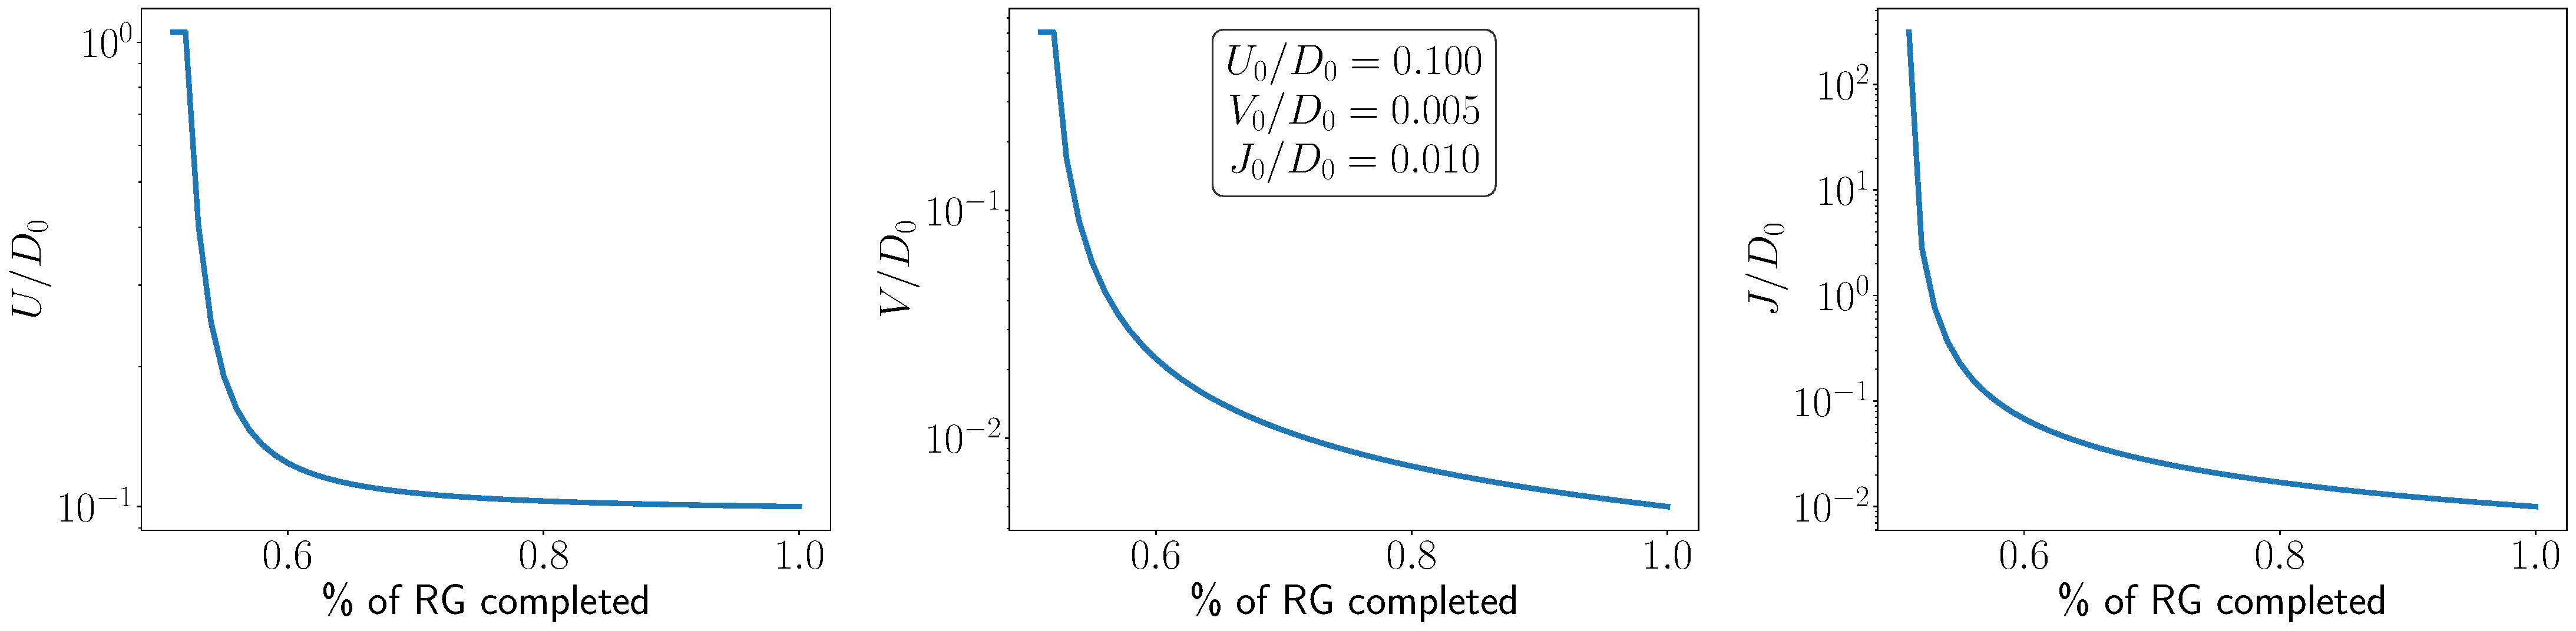
\includegraphics[width=0.99\textwidth]{../spin-charge-symmetrical/U_rel,U_gt_0.pdf}
\end{figure}
\begin{figure}[htpb]
	\centering
	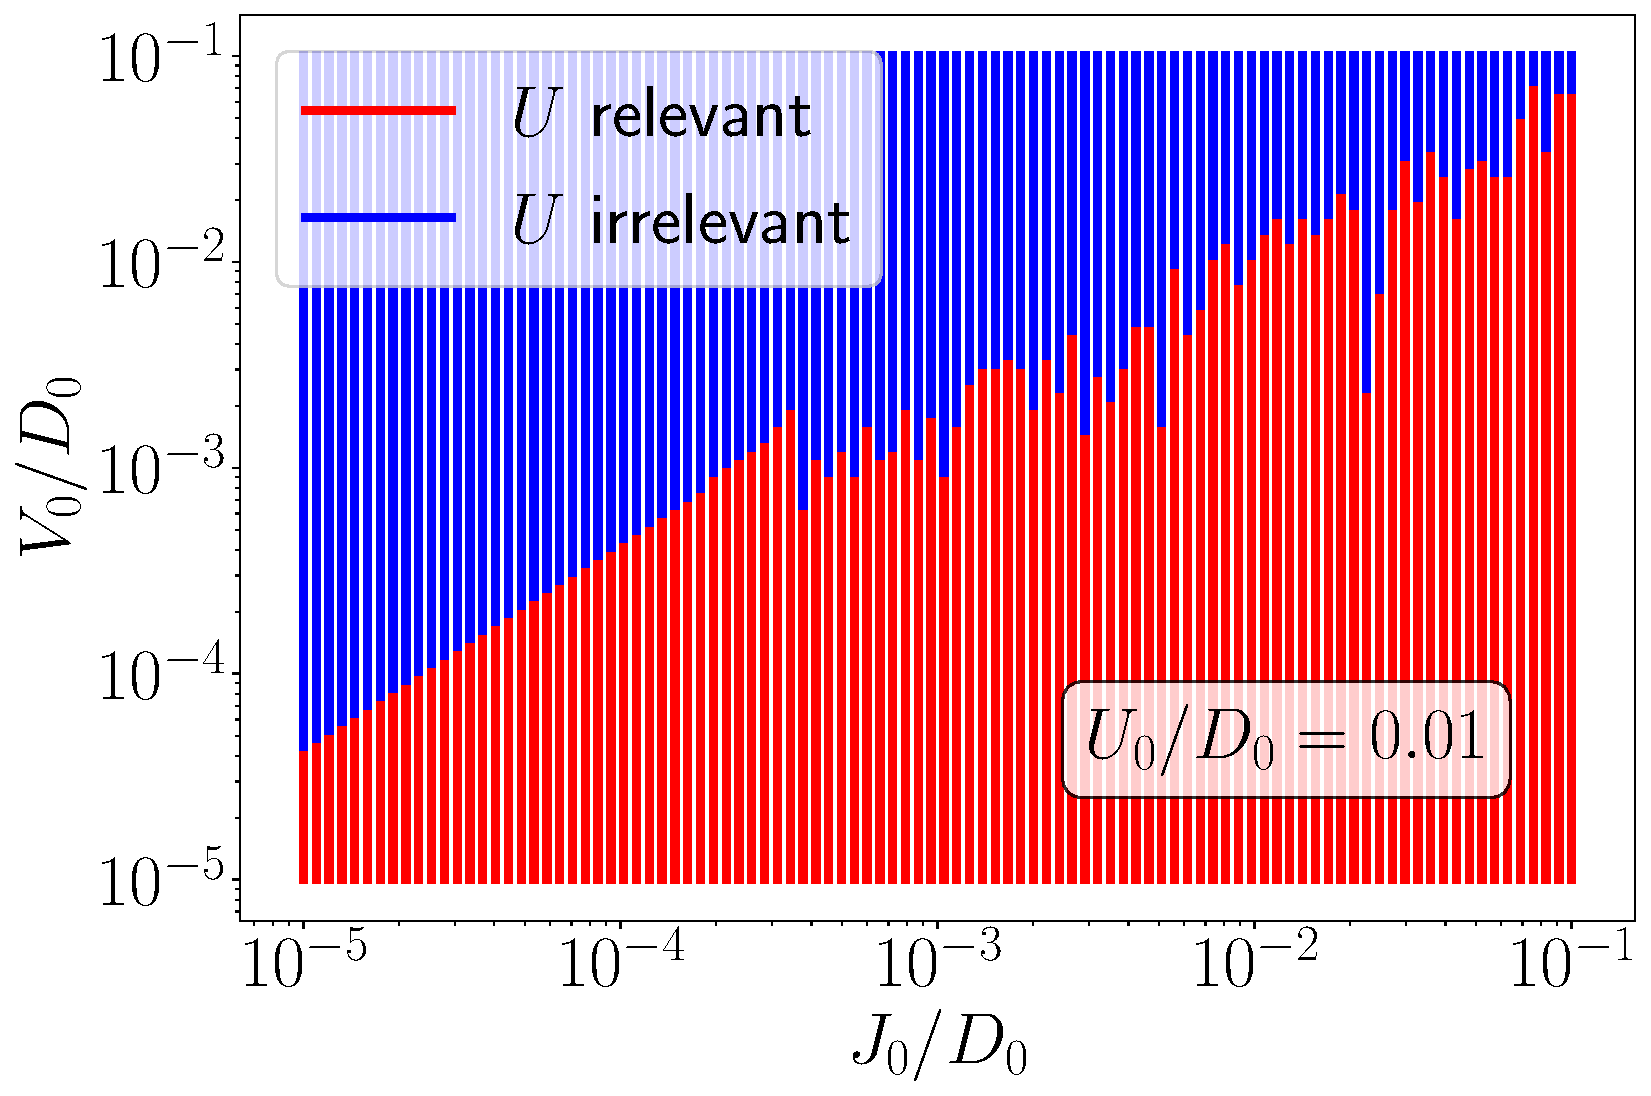
\includegraphics[width=0.48\textwidth]{../spin-charge-symmetrical/VvsJ_relvsirr.pdf}
	\hspace*{\fill}
	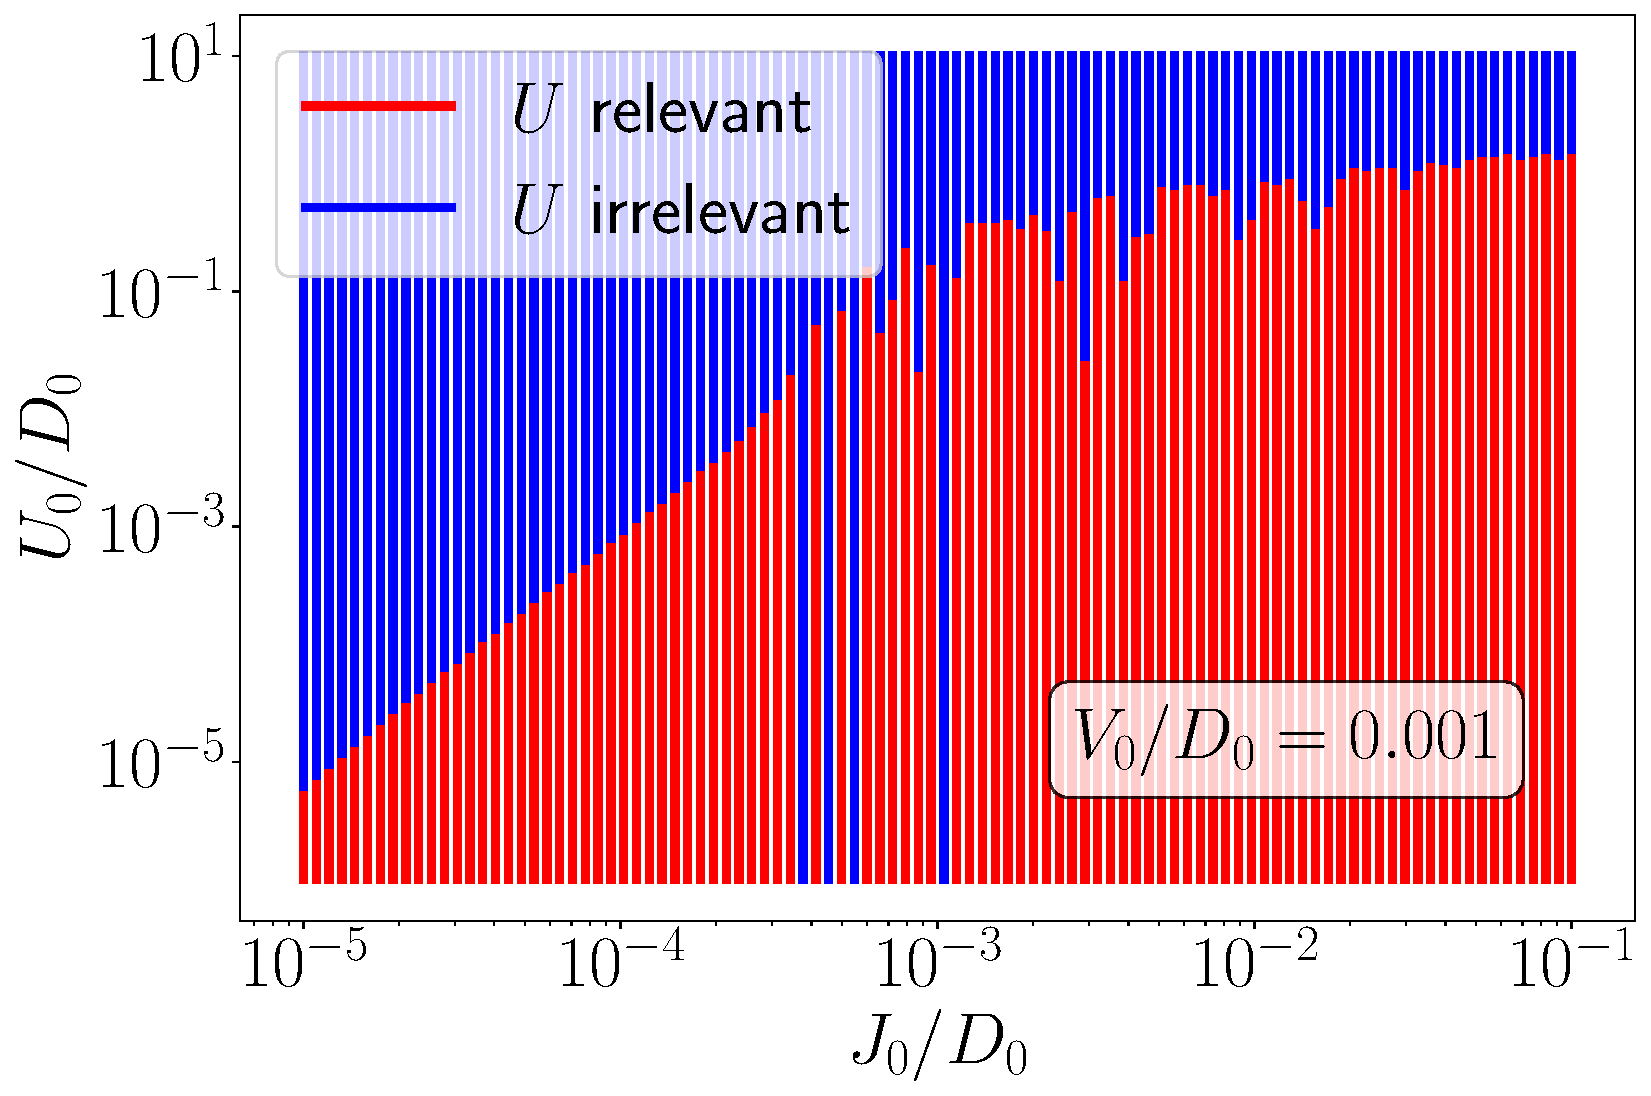
\includegraphics[width=0.48\textwidth]{../spin-charge-symmetrical/UvsJ_relvsirr.pdf}
\end{figure}
\begin{figure}[htpb]
	\centering
	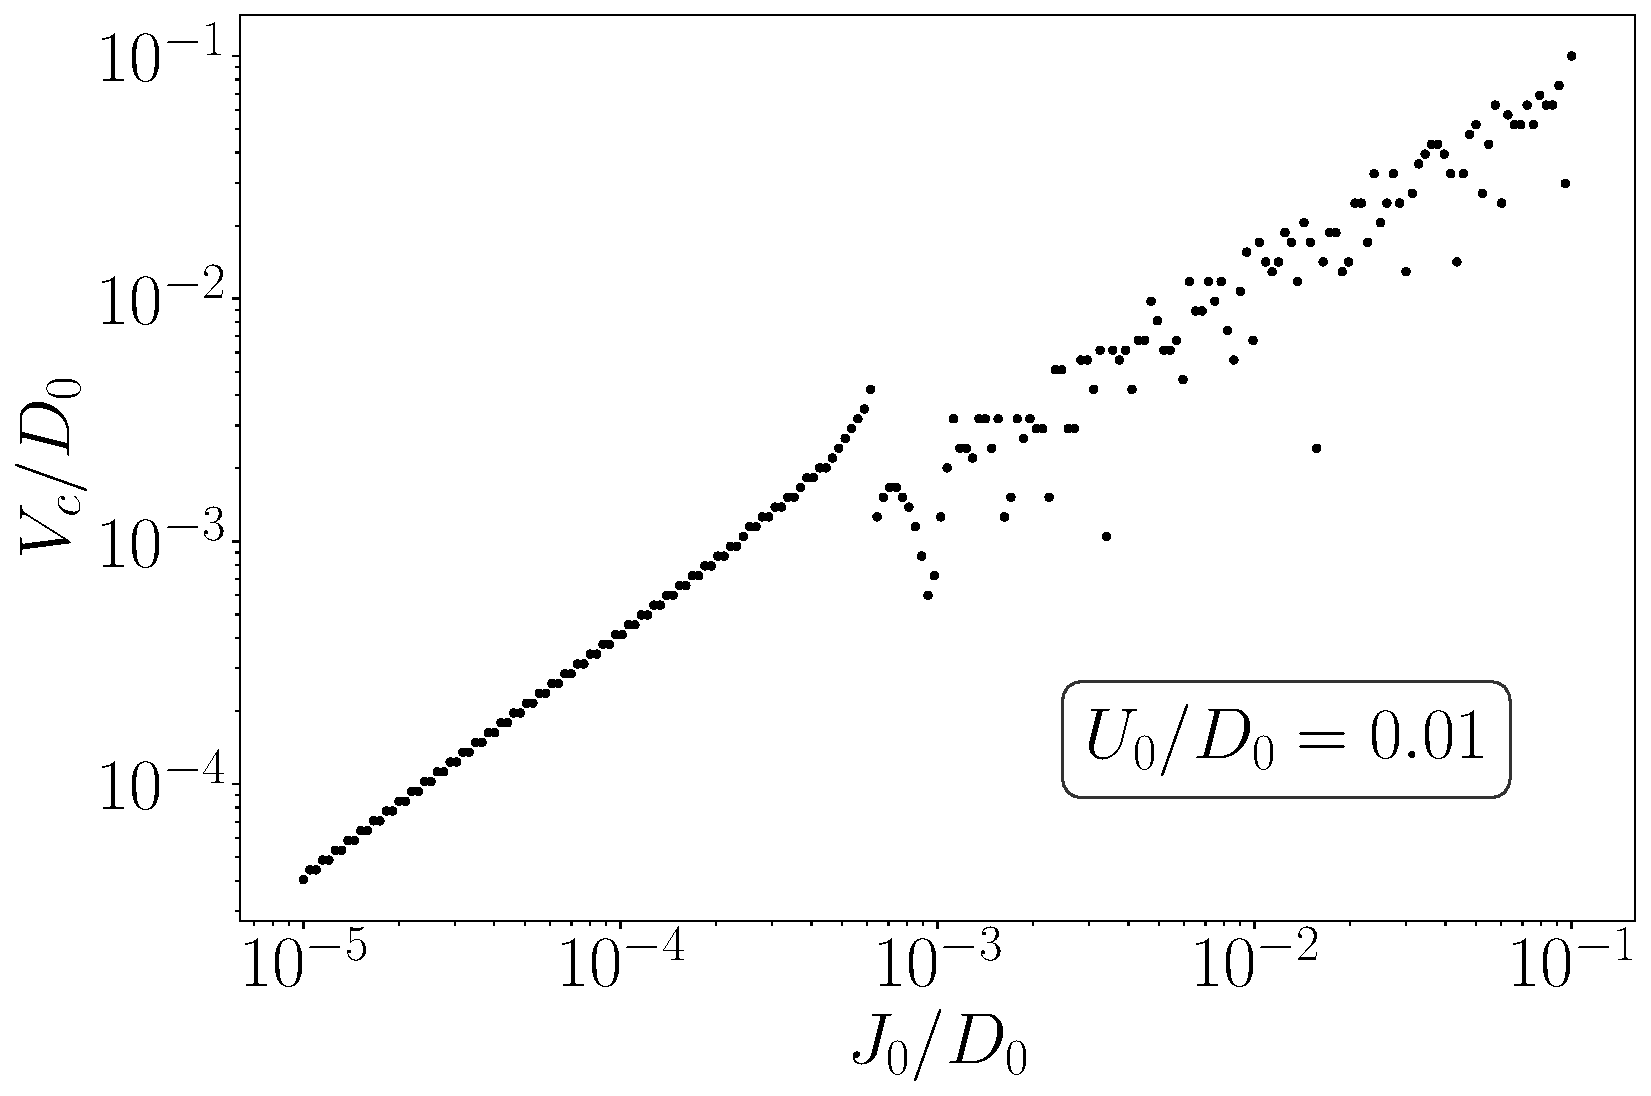
\includegraphics[width=0.48\textwidth]{../spin-charge-symmetrical/VcvsJ.pdf}
	\hspace*{\fill}
	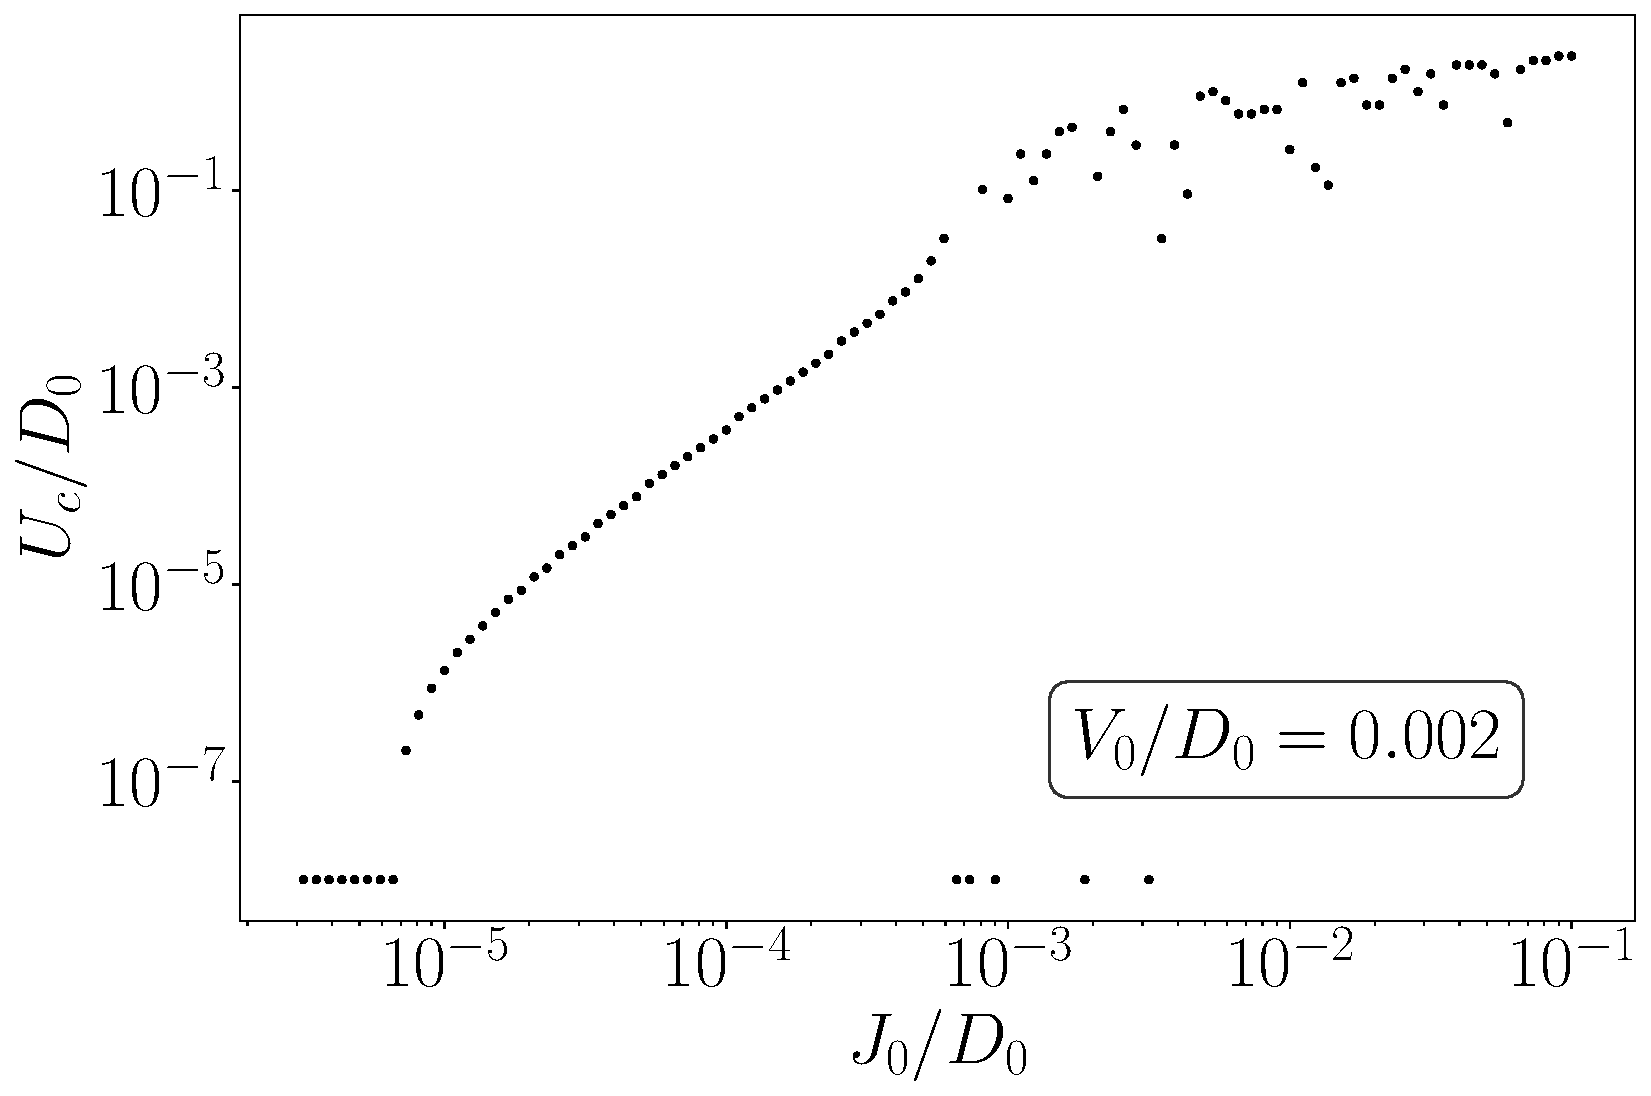
\includegraphics[width=0.48\textwidth]{../spin-charge-symmetrical/UcvsJ.pdf}
	% \caption{../spin-charge-symmetrical/UcvsJ.pdf}
	% \label{fig:-spin-charge-symmetrical-UcvsJ-pdf}
\end{figure}

\section{Nature of RG flows: \(U<0\)}
Here, we have \(J<0\) and \(K>0\). The RG flows in this regime can be exactly mapped on to those in the positive \(U\) regime by transforming \(J \leftrightarrow K\) and \(d_0 \leftrightarrow d_1\).

\section{Effective Hamiltonian and ground state}
The fixed point Hamiltonian can, in general, be written as
\begin{equation}\begin{aligned}
	\mathcal{H}^* = \sum_{\sigma, k}\epsilon_k \tau_{k\sigma} - \frac{U^*}{2}\left(\hat n_{d \uparrow} - \hat n_{d \downarrow}\right)^2  + \sum_{\sigma, k < \Lambda^*}\left( V^* c^\dagger_{k\sigma}c_{d\sigma} + \text{h.c.} \right) + J^* \vec{S_d}\cdot\vec{s} + K^* \vec{C_d}\cdot\vec{C}
\end{aligned}\end{equation}
The first term is the kinetic energy of all the electrons. The next two terms are the impurity-diagonal pieces, featuring the renormalised interaction \(U^*\). The next three terms are the residual interactions between the impurity and the metal, with the renormalised couplings \(V^*, J^*\) and \(K^*\). The summations in these terms extend from the fixed point momentum cutoff \(\Lambda^*\) to 0. This is the region of momentum space  which the URG was unable to decouple. The operators \(\vec s\) and \(\vec C\) represent the macroscopic magnetic and charge spins formed by the remaining electrons that are lying inside the window \(\left[ 0, \Lambda^* \right] \):
\begin{equation}\begin{aligned}
	\vec s = \sum_{kk^\prime<\Lambda^*\atop{\alpha\beta}} c^\dagger_{k\alpha}\vec \sigma_{\alpha\beta}c_{k^\prime\beta}
\end{aligned}\end{equation}
Our goal here is to write down the ground state wavefunction for this low-energy Hamiltonian.

To make progress with the ground state, we will simplify the effective Hamiltonian by mapping it onto a two-site problem. One site is of course the impurity site, and this site will be labeled as site 1. The other site will be formed by the center of mass degree of freedom of the conduction electrons, and will be labeled as site 2. The Hamiltonian for this two-site problem is
\begin{equation}\begin{aligned}
	\mathcal{H}_{IR} = - \frac{U^*}{2}\left(\hat n_{1 \uparrow} - \hat n_{1 \downarrow}\right)^2 + V^*\sum_{\sigma}\left(c^\dagger_{1\sigma}c_{2\sigma} + \text{h.c.} \right) + J^*\vec{S_1}\cdot\vec{S_2} + K^* \vec{C_1}\cdot\vec{C_2}
\end{aligned}\end{equation}
\begin{figure}[!htb]
	\centering
	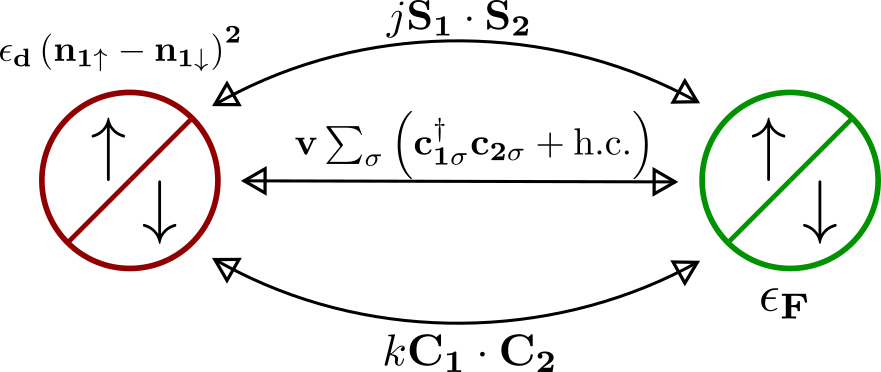
\includegraphics[width=0.4\textwidth]{../figures/two_site_problem.png}
	\caption{Two-site effective problem of fixed point Hamiltonian}
	\label{twosite}

\end{figure}
The subscripts on the operators designate the site on which they act; \(\hat n_1\) is the number operator for the first site.

We will adopt the following notation to represent the states in this Hilbert space. A general state will be represented in the Fock space basis as \(\ket{n_{1 \uparrow}n_{1 \downarrow}n_{2 \uparrow}n_{2 \downarrow}}\). For example,
\begin{equation}\begin{aligned}
	\ket{1101} = c^\dagger_{1 \uparrow}c^\dagger_{1 \downarrow}c^\dagger_{2 \downarrow}\ket{-}
\end{aligned}\end{equation}
\(\ket{-}\) is the vacuum state.

The full list of eigenstates is given in Table~\ref{twosite_spectrum}.
\begin{table}[htb!]
	\centering
	\begin{tabular}{|c|c|c|c|}
		\hline
		\(\hat n\) & \(S_1^z + S_2^z\) & eigenstate & eigenvalue\\
		\hline
		0 & 0 & \(\ket{0,0}\) & \(\frac{1}{4}{K^*}\)\\
		\hline
		4 & 0 & \(\ket{2,2}\) & \(\frac{1}{4}{K^*}\)\\
		\hline
		\multirow{2}{*}{1} & \(\frac{1}{2}\) & \(-4{V^*}\ket{\uparrow,0} +2 \left[-\frac{1}{2}U^* \mp \Delta\left(U^* , {V^*}\right)\right] \ket{0, \uparrow}\) & \multirow{2}{*}{\(-\frac{1}{4}U^* \pm \frac{1}{2}\Delta\left(U^* , {V^*}\right)\)}\\
		 & - \(\frac{1}{2}\) & \(-4{V^*}\ket{\downarrow,0} +2 \left[-\frac{1}{2}U^* \mp \Delta\left(U^* , {V^*}\right)\right] \ket{0, \downarrow}\)  &\\
		\hline
		\multirow{2}{*}{3} & \(\frac{1}{2}\) & \(-4{V^*}\ket{\uparrow,2} +2 \left[-\frac{1}{2}U^* \mp \Delta\left(U^* , {V^*}\right)\right] \ket{2, \uparrow}\) & \multirow{2}{*}{\(-\frac{1}{4}U^* \pm \frac{1}{2}\Delta\left(U^* , {V^*}\right)\)}\\
		 & - \(\frac{1}{2}\) & \(-4{V^*}\ket{\downarrow,2} +2 \left[-\frac{1}{2}U^* \mp \Delta\left(U^* , {V^*}\right)\right] \ket{2, \downarrow}\)  &\\
		\hline
		\multirow{3}{*}{2} & 1,-1,0 & \(\ket{\uparrow,\uparrow}\), \(\ket{\downarrow,\downarrow}\), \(\ket{\uparrow,\downarrow} + \ket{\downarrow, \uparrow}\) & {\(-\frac{1}{2}U^* + \frac{1}{4}{J^*}\)}\\
		\cline{2-4}
		& 0 & \(\ket{2,0} - \ket{0,2}\) & \(-\frac{3}{4}{K^*}\)\\
		\cline{2-4}
		& 0 & \(c_\pm^s \frac{1}{\sqrt 2}\left(\ket{\uparrow, \downarrow} - \ket{\downarrow, \uparrow}\right) + c^c_\pm \frac{1}{\sqrt 2}\left(\ket{\uparrow\downarrow, 0} + \ket{0, \uparrow\downarrow}\right)\) & \({V^*}\left[ \gamma \pm \sqrt{\gamma^2 + 4} \right] -\frac{1}{2}U^* - \frac{3}{4}{J^*}\)\\
		\hline
	\end{tabular}
	\caption{Eigenstates for effective two-site Hamiltonian}
	\label{twosite_spectrum}
\end{table}
The quantities \(\Delta\) and \(\gamma\) are defined as
\begin{equation}\begin{aligned}
	\label{gamma_def}
	\Delta\left(U^*, V^*\right) = \frac{1}{2}\sqrt{{U^*}^2 + 16{V^*}^2}, \quad \gamma = \frac{1}{2{V^*}}\left[ \frac{1}{4}\left( 3J^* + K^* \right) + \frac{1}{2}U^* \right] 
\end{aligned}\end{equation}
and the coefficients \(c^{s,c}_\pm\) for the last eigenstate are given by
\begin{equation}\begin{aligned}
	c^s_\pm = \frac{1}{\sqrt{2\sqrt{\gamma^2 + 4}}}\sqrt{\sqrt{\gamma^2 + 4} \mp \gamma} = \mp c^c_\mp
\end{aligned}\end{equation}

For \(U>0\), the ground state is given by
\begin{gather}
	\ket{\Psi}_\text{gs} = c_\pm^s \frac{1}{\sqrt 2}\left(\ket{\uparrow, \downarrow} - \ket{\downarrow, \uparrow}\right) + c^c_\pm \frac{1}{\sqrt 2}\left(\ket{\uparrow\downarrow, 0} + \ket{0, \uparrow\downarrow}\right), \quad E_\text{gs} =  -V^*\sqrt{\gamma^2 + 4} -\frac{1}{4}U^* - \frac{3}{8}{J^*}
\end{gather}

The probabilities for the spin and charge sectors for the ground state are
\begin{equation}\begin{aligned}
	\left( c^s_- \right)^2 = \frac{1}{2\sqrt{\gamma^2 + 4}}\left(\sqrt{\gamma^2 + 4} + \gamma\right), \quad \left( c^c_- \right)^2 = \frac{1}{2\sqrt{\gamma^2 + 4}}\left(\sqrt{\gamma^2 + 4} - \gamma\right)~.
\end{aligned}\end{equation}
For (roughly) \(J_0 > V_0\), we get \(J^* \gg V^*\) and \(U^* \gg U_0\) so that \(\gamma \gg 1\). This gives \(\left( c^s_- \right) ^2 \sim 1\) and \(\left( c^c_- \right) ^2 \sim 0\). The entire contribution to the ground state then comes from the spin sectors of the two sites. This is calculated numerically in fig.~\ref{cs_cc}.
\begin{figure}[htpb]
	\centering
	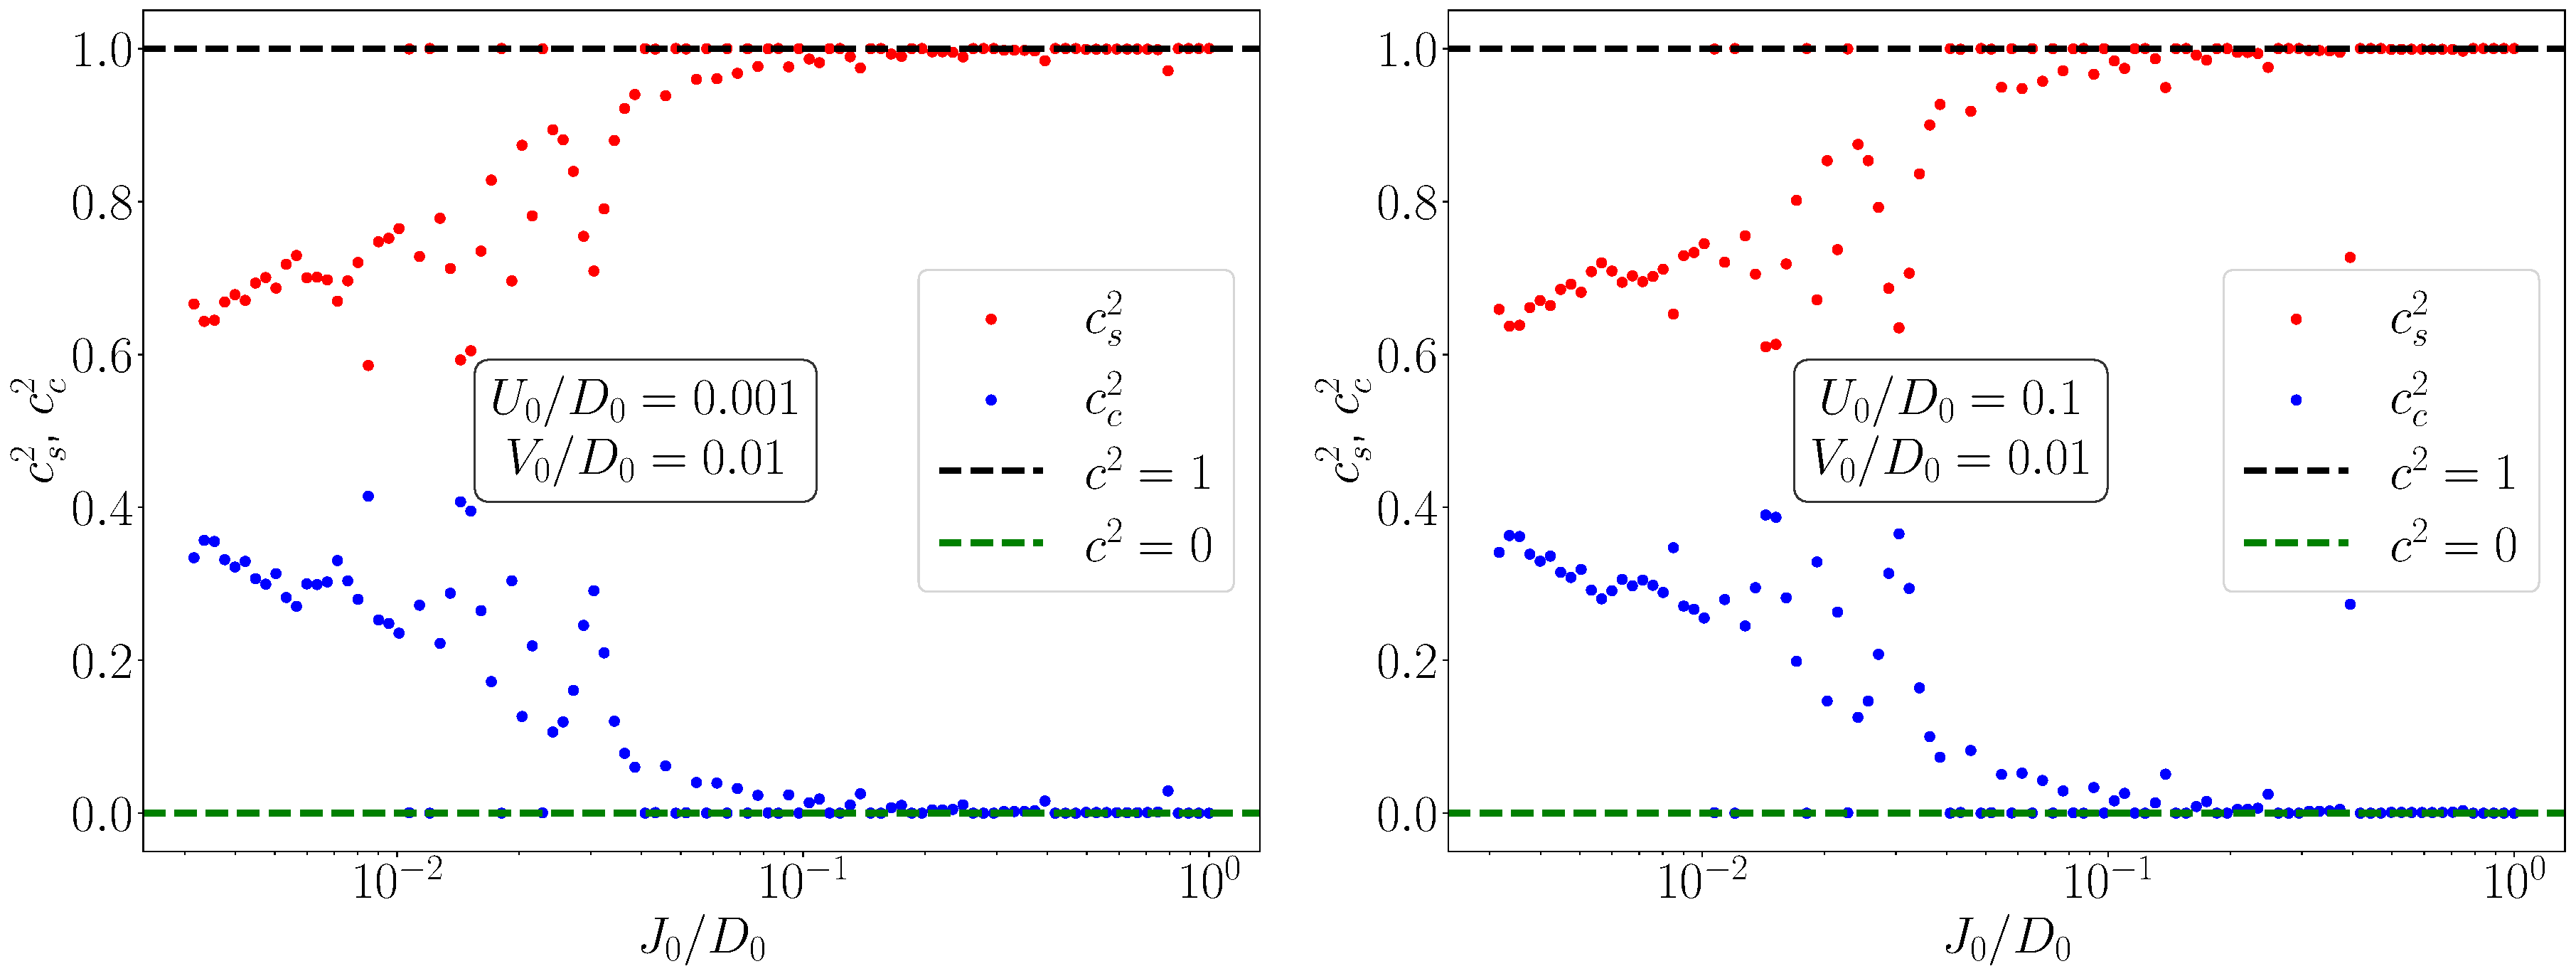
\includegraphics[width=0.8\textwidth]{../spin-charge-symmetrical/coeffs_vs_J.pdf}
	\caption{Variation of relative weights \(c^s_-\) and \(c^c_-\) with \(J_0\)}
	\label{cs_cc}
\end{figure}

\section{Effective temperature scale at the fixed point}
We will first change the discrete RG equation to a continuum equation by interpreting \(\Delta J\) as \(\frac{\Delta J}{\Delta \ln D}\), where the denominator is unity: \(\Delta \ln D = 1\). Now, since the bandwidth is decreasing under the RG, we can write \(\Delta \ln D = -d \ln D\). The continuum equation (for \(K=0\)) becomes
\begin{equation}\begin{aligned}
	\frac{\:\mathrm{d}J}{\:\mathrm{d}\ln D} = n(0)J^2 \frac{1}{\omega - \frac{D}{2} + \frac{J}{4}}
\end{aligned}\end{equation}
where we have replaced by the number of states at each shell with that at the Fermi surface (uniform DOS). We can define a dimensionless quantity \(g \equiv \frac{J}{\frac{D}{2}} - \omega\). In terms of \(g\), the continuum RG equation becomes
\begin{equation}\begin{aligned}
	-\frac{\:\mathrm{d}g}{\:\mathrm{d}\ln D} + \frac{D g}{2\omega - D} = \frac{n(0) g^2}{1 - \frac{g}{4}}
\end{aligned}\end{equation}
Now, for the specific case where \(D\) is small (\(D \to 0\)), we can simplify and integrate this equation:
\begin{equation}\begin{aligned}
	\frac{\:\mathrm{d}g}{\:\mathrm{d}\ln D} &= \frac{n(0) g^2}{\frac{g}{4} - 1}\\
	\implies \left[\frac{1}{g} + \frac{1}{4}\ln g\right]_{g_0}^{g^*} &= n(0)\ln D\big\vert_{D_0}^{D^*}
\end{aligned}\end{equation}
\(g^*(_0), D^*(_0)\) are the fixed point (bare) values of \(g, D\). From the denominator structure, the fixed-point value is \(g^* =  4\). This gives an estimate of the bandwidth of the emergent window:
\begin{equation}\begin{aligned}
	D^* = D_0 \left( \frac{4}{g_0} \right)^\frac{1}{4n(0)}\exp\left\{-\frac{1}{n(0)}\left(\frac{1}{g_0} - \frac{1}{4}\right)\right\}
\end{aligned}\end{equation}
We can now define a temperature scale for the fixed-point theory:
\begin{equation}\begin{aligned}
	T_K \equiv \frac{2N^*}{\pi}D^* = \frac{2N^*}{\pi}D_0 \left( \frac{4}{g_0} \right)^\frac{1}{4n(0)}\exp\left\{-\frac{1}{n(0)}\left(\frac{1}{g_0} - \frac{1}{4}\right)\right\}
\end{aligned}\end{equation}
The factor of \(2N^*\) is inserted to make the Kondo temperature intensive (we will see below that the \(N^*\) allows it to  be written in terms of parameters of the two-site Hamiltonian) - \(2N^*\) is the total number of momentum states in the fixed point theory. The factor of \(\frac{1}{\pi}\) is for aesthetic reasons. Since we have and will primarily work with \(\omega=0\), the fixed point condition can be used to write \(D^* = \frac{J^* + K^*}{2}\).
\begin{equation}\begin{aligned}
	T_K = \frac{2N^*}{\pi}\frac{1}{2}\left(J^* + K^*\right) = \frac{1}{\pi}\left(j + k\right)
\end{aligned}\end{equation}
